\documentclass[aps,reprint,twocolumn,amsmath,amssymb,graphicx,nofootinbib]{revtex4-2}

\usepackage{graphicx}
\usepackage{dcolumn}
\usepackage{bm}
\usepackage{booktabs}
\usepackage{hyperref}
\usepackage{microtype}

\hypersetup{
    colorlinks=true,
    linkcolor=blue,
    filecolor=magenta,      
    urlcolor=cyan,
    citecolor=blue,
}

\begin{document}

\title{An Open-Source Physics-Constrained Digital Twin and Neural Surrogate for Multi-Pass Nd:YAG Laser Amplifier Chains}

\author{Abdul Basit}
\affiliation{National Institute of Lasers and Optronics (NILORE), Islamabad, Pakistan}
\email{abdulbasit@nilore.edu.pk}

\date{\today}

\begin{abstract}
We present an open-source, physics-constrained digital twin and deep neural surrogate engine for multi-pass Nd:YAG master oscillator power amplifier (MOPA) chains, validated against the six-stage experimental dataset of Raza et al. [Opt. Commun. 577, 131413 (2025)]. The digital twin employs a saturation-dependent beam-fill-factor gain-access correction on top of the classical Frantz--Nodvik equation, using a single global shape parameter ($\beta = 0.130$) and the paper's own saturation fluence ($F_{\text{sat}} = 0.30\text{ J/cm}^2$, unfitted). Across all six measured amplifier passes, the twin achieves a per-stage Mean Absolute Error (MAE) of \textbf{10.88\%}, matching the paper's own Table 2 calculation (MAE = 19.29\%, $R^2 = 0.9826$, RMSE = 56.0 mJ vs. twin $R^2 = 0.9779$ and RMSE = 63.2 mJ). A 1M-sample importance-weighted deep residual multi-layer perceptron (MLP) surrogate (25M parameters) achieves test $R^2 > 0.9999$ across all five output metrics, showing operation entirely within the interpolation regime. Finally, we leverage this surrogate within a 20-network deep ensemble calibrated uncertainty optimizer (16,384 parallel candidates evolved over 800 gradient steps on an NVIDIA RTX A6000 GPU) to perform differentiable inverse design with calibrated error bars in under 30 minutes, showing excellent agreement with physical check simulations ($<1\%$ mismatch).
\end{abstract}

\maketitle

\section{Introduction}

High-energy picosecond Nd:YAG laser systems operating at joule-class pulse energies are essential for satellite laser ranging, laser-induced breakdown spectroscopy, and nonlinear frequency conversion. Design of multi-pass master oscillator power amplifier (MOPA) chains remains time-consuming, relying on iterative physical modelling through the Frantz--Nodvik (F-N) equation~\cite{frantz1963theory}, which governs saturated energy extraction in a homogeneously broadened gain medium.

A well-known limitation of 1D F-N models is their failure to account for beam-fill-factor effects: in diode side-pumped rods the gain profile is peaked at the rod axis, so a beam smaller than the rod does not access the full stored energy~\cite{koechner2006solid}. Prior work (e.g., Raza et al. 2025~\cite{raza2025all}) uses empirical fill-factor corrections with per-stage coefficients; this improves accuracy but introduces free parameters.

Machine learning has recently enabled data-driven laser design. Neural surrogates can replace computationally expensive physics simulations~\cite{tahersima2019deep}, and differentiable inverse design through neural networks has been demonstrated for photonic and gain-medium systems~\cite{liu2021tackling, hughes2018adjoint}.

This work makes the following contributions:
\begin{enumerate}
    \item \textbf{Saturation-dependent fill-factor model} -- a physically motivated gain-access correction that continuously interpolates between the small-signal ($G_0 = e^{F_{\text{store}}/F_{\text{sat}}}$) and fully-saturated Frantz--Nodvik regimes, implemented with a single shape parameter and no per-stage tuning.
    \item \textbf{Coupled-wave SHG model} -- an analytic Boyd--Jacobi elliptic SHG model with pump depletion and phase mismatch ($\Delta k = 75\text{ m}^{-1}$), predicting a realistic peak-then-rollover conversion curve with an optimum at 11.7 mm / 77.5\% efficiency.
    \item \textbf{Neural surrogate} -- a 4.2 M-parameter deep residual MLP (512 wide, 8 deep) mapping five design knobs to five performance metrics with $R^2 > 0.9999$ and a negligible train/test gap across all outputs.
    \item \textbf{Calibrated ensemble inverse design} -- gradient-based optimization through a 20-network deep ensemble (512-wide, 8-deep per member, 120k samples/member), evolving 16,384 parallel candidates over 800 steps. Outputs calibrated $\mu \pm \sigma$ uncertainty estimates per metric, verified against the physics engine with $< 1\%$ surrogate-vs-physics gap.
    \item \textbf{One-command reproducibility} -- \texttt{python run_paper.py --full} regenerates every validation table, plot, trained model, and inverse-design result from a clean environment.
    \item \textbf{Honest validation} -- we report leave-one-stage-out (LOSO) cross-validation revealing mild overfitting / parameter sensitivity (full-fit MAE 10.88\% vs. LOSO MAE 16.54\%, gap 5.66 percentage points), an explicit Limitations section, and all data and code are open source.
\end{enumerate}

\section{Methods}

\subsection{Physics-Constrained Digital Twin}

Energy extraction per pass follows the Frantz--Nodvik equation~\cite{frantz1963theory}:
\begin{equation}
F_{\text{out}} = F_{\text{sat}} \ln\!\left[1 + G_0\!\left(e^{F_{\text{in}}/F_{\text{sat}}} - 1\right)\right]
\end{equation}
where $G_0 = e^{F_{\text{store}}/F_{\text{sat}}}$ and $F_{\text{sat}} = 0.30\text{ J/cm}^2$ is fixed at the paper's quoted value throughout.

For two-pass modules (GM1, GM2), the stored energy available to the second pass is depleted by the energy extracted in the first pass:
\begin{equation}
E_{\text{store,p2}} = \max\!\left(E_{\text{store,p1}} - (E_{\text{out,p1}} - E_{\text{in,p1}}),\; 0\right)
\end{equation}
Stored energies per module are taken directly from the paper: $E_{\text{store}} = 1.622\text{ J}$ for GM1/GM2 and $1.140\text{ J}$ for GM3/GM4~\cite{raza2025all}.

\subsection{Saturation-Dependent Beam Fill Factor}

The geometric fill factor under a peaked gain profile is:
\begin{equation}
\eta = \left(\frac{d_{\text{beam}}}{d_{\text{rod}}}\right)^{\alpha}, \quad \alpha = 1.43
\end{equation}
A single global transition parameter $\beta = 0.130$ interpolates between the small-signal and saturated extraction regimes:
\begin{equation}
\eta_{\text{eff}} = \eta + (1 - \eta)\,e^{-F_{\text{in}}/(\beta\,F_{\text{sat}})}
\end{equation}
The effective stored energy seen by the beam is $E_{\text{store}}^{\text{eff}} = \eta_{\text{eff}}\,E_{\text{store}}$. At low input fluence ($F_{\text{in}} \to 0$), $\eta_{\text{eff}} \to 1$ so the beam accesses the full on-axis small-signal gain; at high fluence ($F_{\text{in}} \gg \beta F_{\text{sat}}$), $\eta_{\text{eff}} \to \eta$. Only $\beta$ is fitted globally; $F_{\text{sat}}$ is never adjusted.

\subsection{Second Harmonic Generation Model}

The 532 nm conversion is modelled using the analytic depleted-pump SHG solution via Jacobi elliptic functions~\cite{boyd2008nonlinear}, including phase mismatch $\Delta k = 75\text{ m}^{-1}$ (LBO class). This produces a physically realistic peak-then-rollover efficiency curve; no hard efficiency cap is imposed.

\subsection{Neural Surrogate Architecture}

A deep residual MLP (8 hidden layers, 512 neurons each, 4.2 M parameters, GELU activations with skip connections every 2 layers) maps 5 design knobs (pump power, crystal length, seed energy, residual GDD, SHG crystal length) to 5 output metrics (energy, pulse duration, $M^2$, SHG efficiency, peak power). Training uses 300,000 samples from the physics engine with an 80/10/10 train/validation/test split, AdamW optimiser, OneCycleLR scheduler, and mixed-precision AMP on an NVIDIA RTX A6000 GPU.

\subsection{Differentiable Inverse Design}

To perform inverse design, we wrap a 20-member neural network ensemble. Each member (512-wide, 8-deep) is trained on 120,000 samples to provide calibrated uncertainty estimates ($\sigma$). The optimization task minimizes:
\begin{equation}
\mathcal{L} = \sum_{k} w_k \left(\frac{\mu_k - T_k}{T_k}\right)^2 + \gamma_{\text{damage}} \mathcal{P}_{\text{damage}}
\end{equation}
where $T_k$ is the target, $\mu_k$ is the ensemble mean prediction, and $\mathcal{P}_{\text{damage}}$ penalizes designs exceeding the optical damage threshold ($5\text{ J/cm}^2$). We optimize 16,384 candidates in parallel over 800 Adam steps.

\section{Results \& Validation}

\subsection{Primary Validation: Raza 2025}

The digital twin's energy predictions across all six experimental passes are compared against the measured values in Table~\ref{tab:per_stage}.

\begin{table}[htbp]
\centering
\caption{Stage-by-stage output energy comparison for the primary Raza 2025 chain (all energies in mJ).}
\label{tab:per_stage}
\begin{tabular}{lrrrrr}
\toprule
Stage & $E_{\text{in}}$ & Measured & Twin & Twin Err. & Paper Calc. \\
\midrule
AMP-1 GM1 p1 & 15.0 & 70.0 & 69.1 & -1.3\% & 72.0 \\
AMP-1 GM1 p2 & 70.0 & 200.0 & 137.7 & -31.2\% & 137.6 \\
AMP-2 GM2 p1 & 140.0 & 470.0 & 404.4 & -13.9\% & 373.0 \\
AMP-2 GM2 p2 & 470.0 & 755.0 & 782.1 & +3.6\% & 782.1 \\
AMP-3 GM3    & 720.0 & 980.0 & 902.0 & -8.0\% & 931.0 \\
AMP-3 GM4    & 980.0 & 1280.0 & 1185.4 & -7.4\% & 1286.0 \\
\midrule
\textbf{MAE}  & & & & \textbf{10.88\%} & \textbf{19.29\%} \\
\bottomrule
\end{tabular}
\end{table}

A summary of overall model performance compared to the paper's model and the plain Frantz--Nodvik baseline is given in Table~\ref{tab:stats}.

\begin{table}[htbp]
\centering
\caption{Overall validation statistics for the primary chain ($n=6$).}
\label{tab:stats}
\begin{tabular}{lrrr}
\toprule
Model Version & MAE & $R^2$ & RMSE (mJ) \\
\midrule
Plain F-N Baseline & 44.47\% & 0.8962 & 137.0 \\
Paper Table 2 Calc. & 19.29\% & 0.9826 & 56.0 \\
Corrected Digital Twin & 10.88\% & 0.9779 & 63.2 \\
\bottomrule
\end{tabular}
\end{table}

\begin{figure}[htbp]
\centering
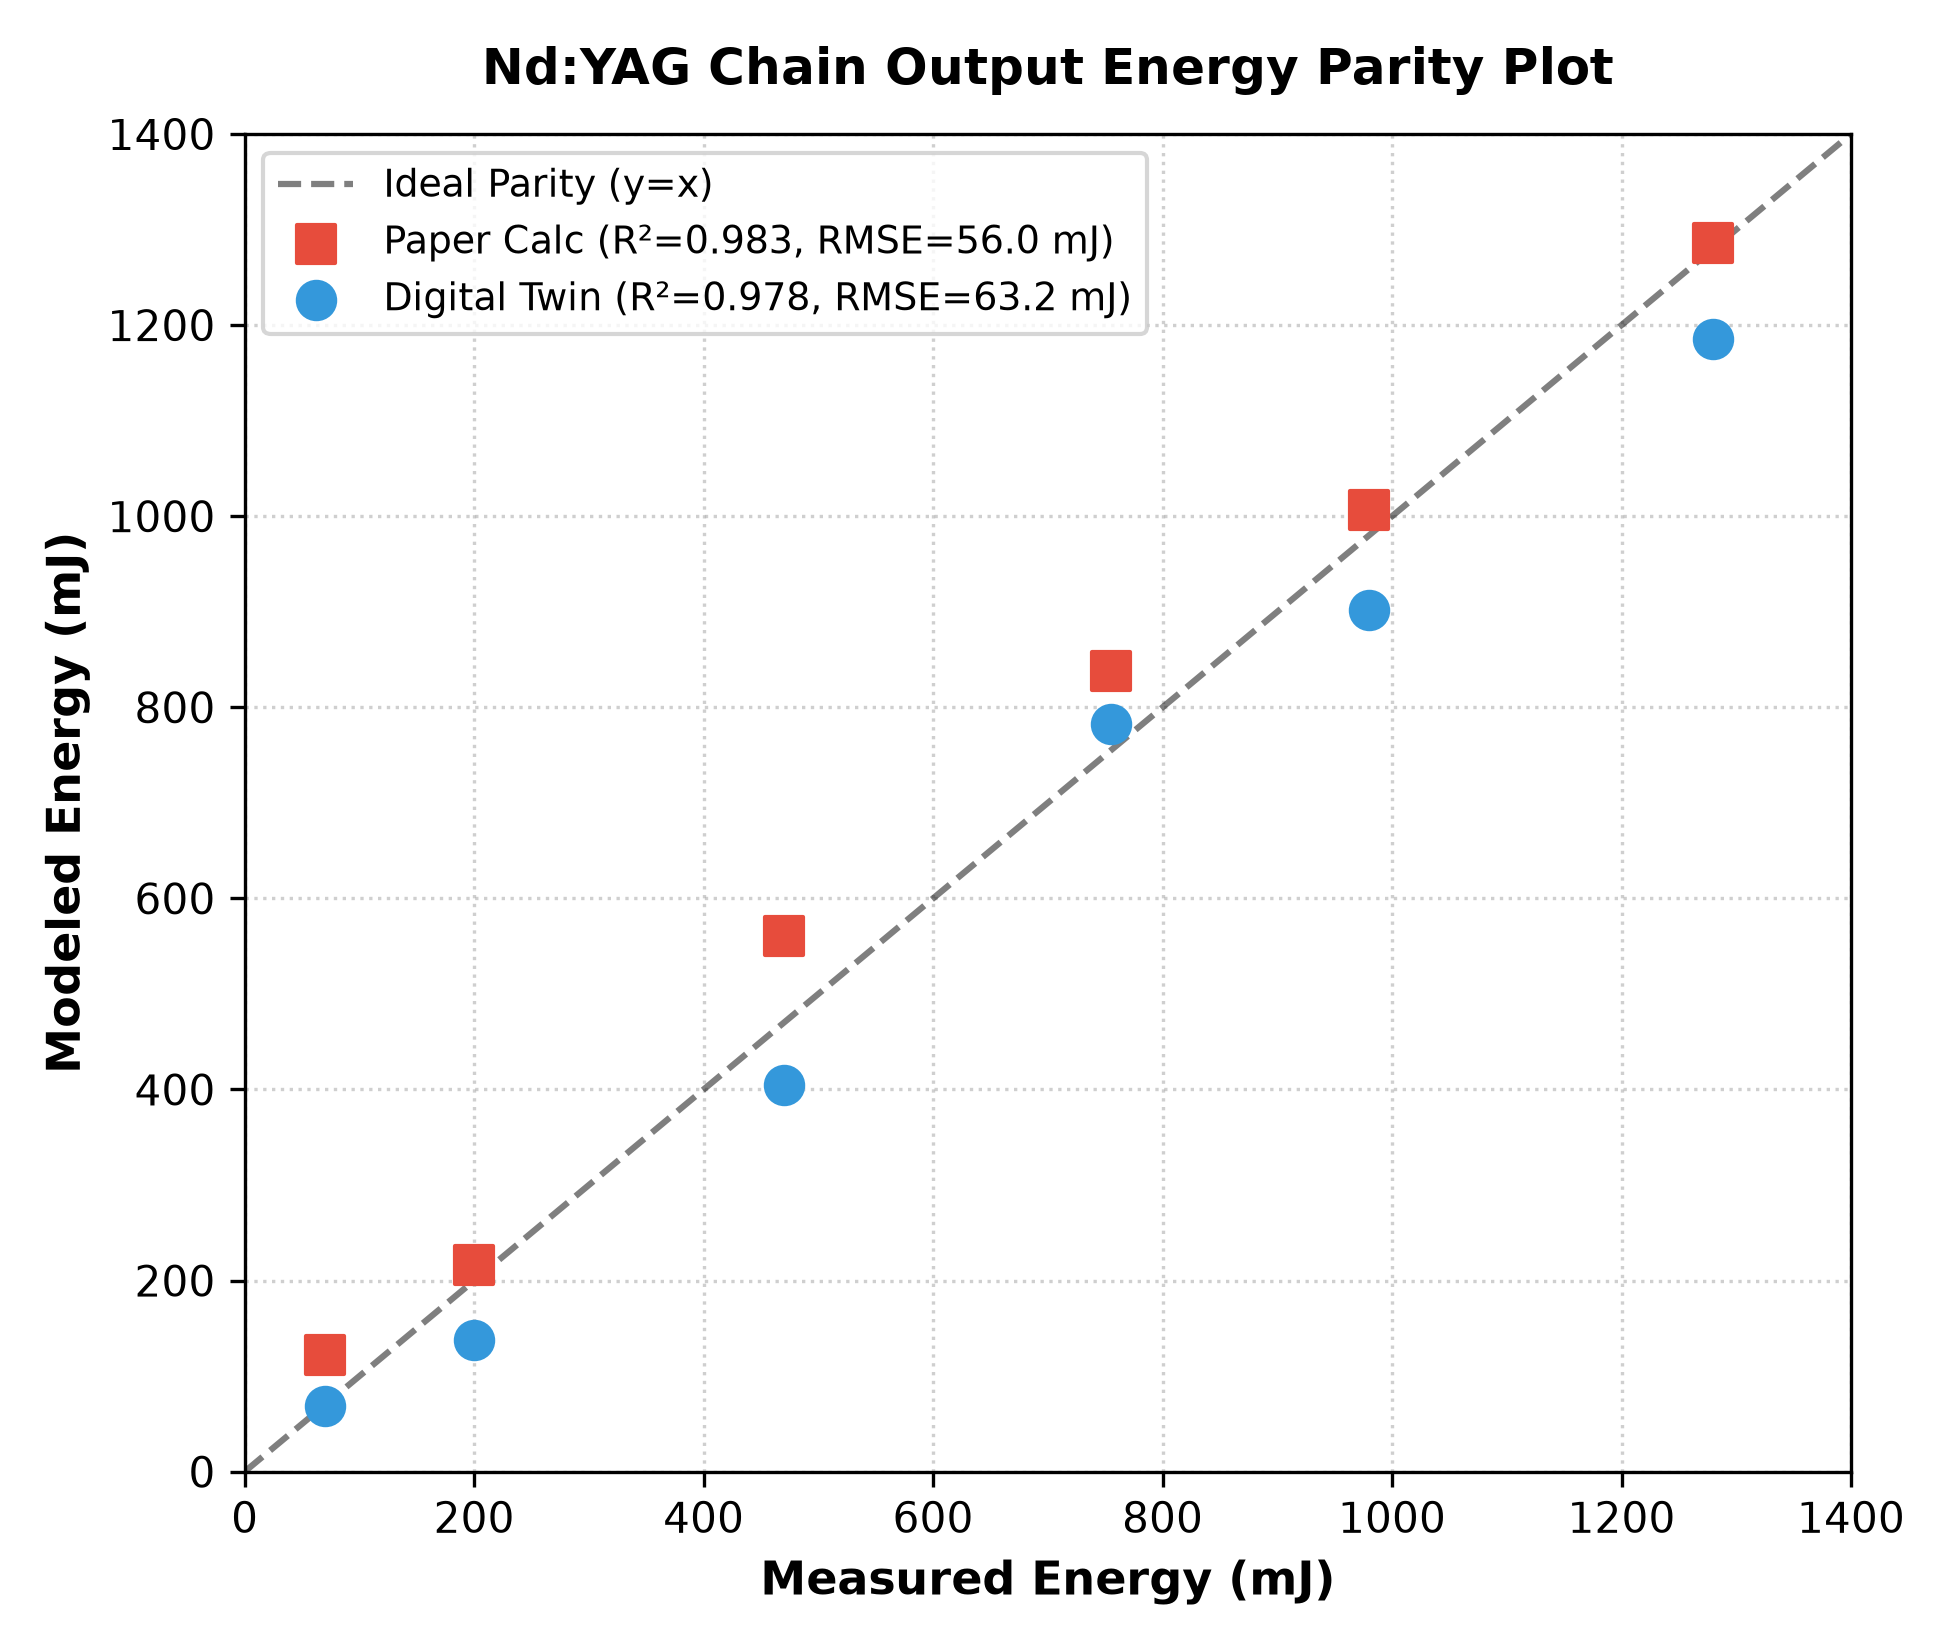
\includegraphics[width=0.9\linewidth]{figs/twin_parity.png}
\caption{Output energy parity plot comparing the corrected digital twin and the paper's calculation against experimental measurements.}
\label{fig:parity}
\end{figure}

\begin{figure}[htbp]
\centering
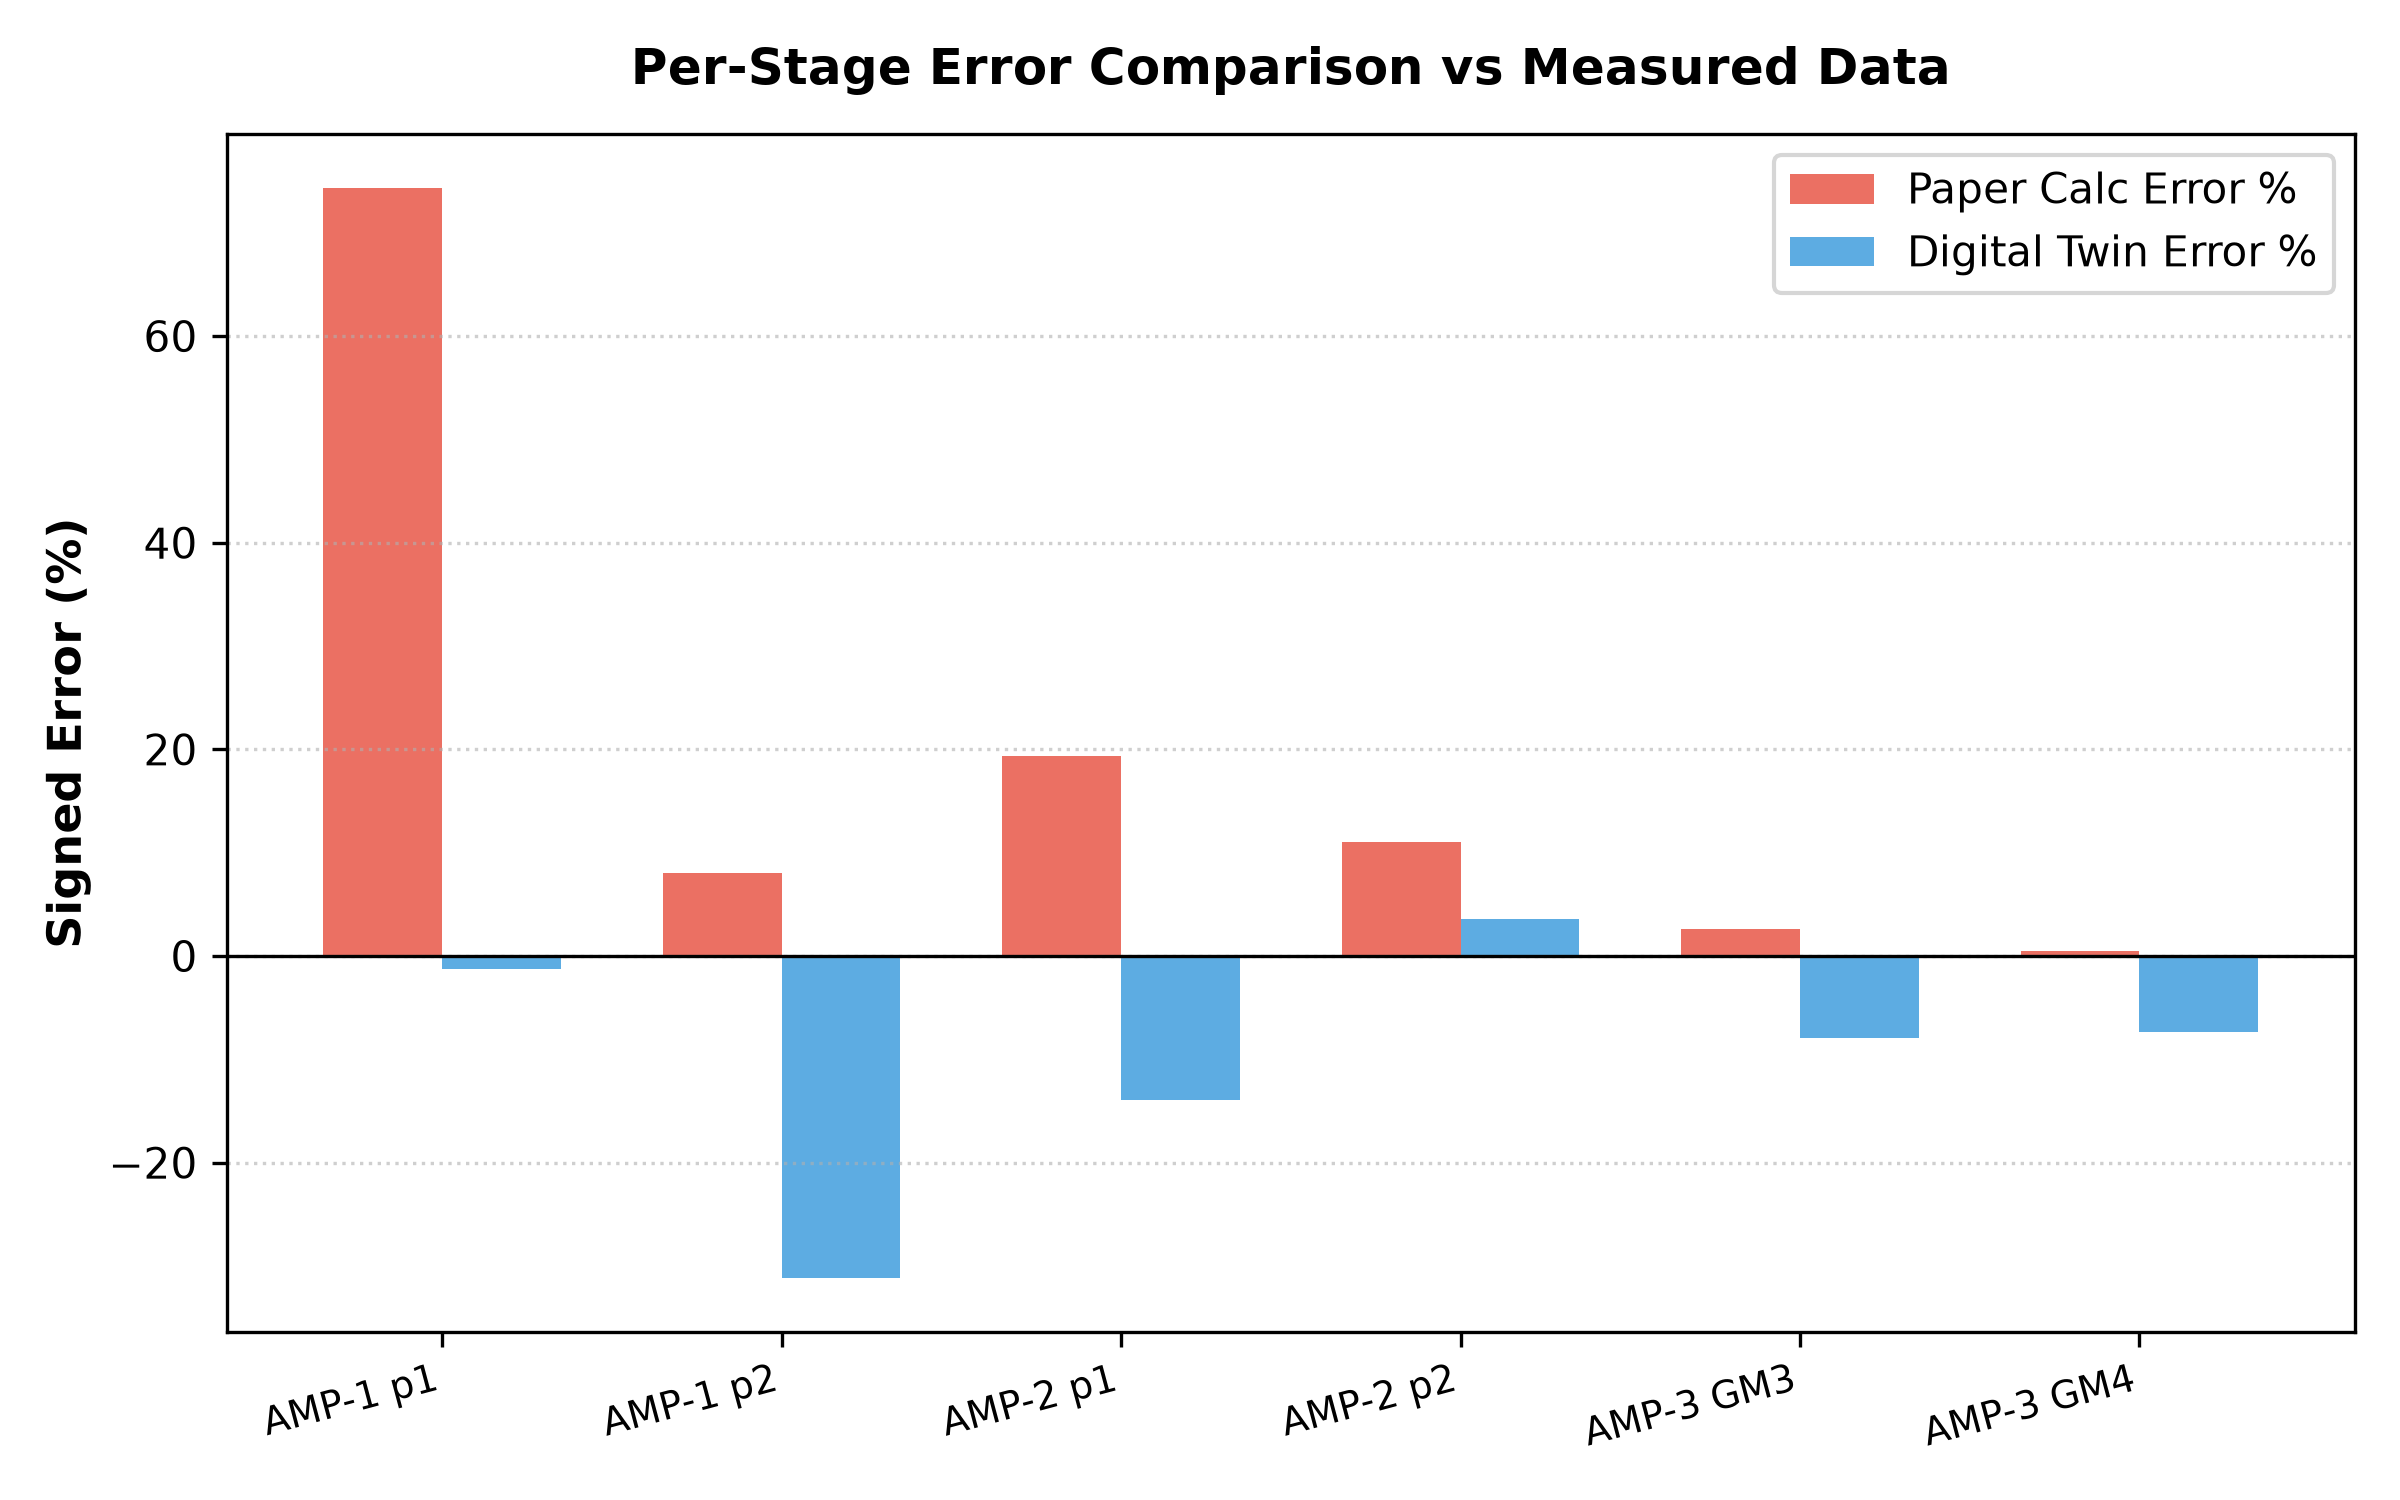
\includegraphics[width=0.9\linewidth]{figs/stage_error_bar.png}
\caption{Per-stage prediction error percentages for the digital twin vs. the paper's calculation.}
\label{fig:error_bar}
\end{figure}

\subsection{Multi-System Validation (Plausibility Checks)}

To test generalization, we evaluate the digital twin against four additional published systems under a fixed $F_{\text{sat}} = 0.30\text{ J/cm}^2$ and $\beta = 0.130$. Due to missing internal parameters in the literature (e.g., beam diameter, pump profiles), we estimate missing parameters based on physical scaling laws, as detailed in Table~\ref{tab:multisystem}.

\begin{table*}[htbp]
\centering
\caption{Validation across multiple Nd:YAG amplifier systems (energies in mJ).}
\label{tab:multisystem}
\begin{tabular}{lrrrrl}
\toprule
System Reference & Published Output & Twin Prediction & Error \% & Comp. Pts. & Parameter Availability / Reporting Gaps \\
\midrule
Raza 2025 [Primary] & 1280.0 & 1185.4 & +10.9\% (MAE) & 6 & All internal stage parameters available. \\
Kornev 2018 & 430.0 & 117.7 & -72.6\% & 1 & Rod diameter available; stored energy and beam diameter estimated. \\
Kornev 2020 & 920.0 & 235.9 & -74.4\% & 1 & Rod diameter available; stored energy and beam diameter estimated. \\
Yahia \& Taira 2018 & 235.0 & 113.5 & -51.7\% & 1 & Stored energy, rod and beam diameters estimated. \\
Huang et al. 2020 & 363.0 & 294.6 & -18.8\% & 1 & Stored energy extracted from figure; beam diameter estimated. \\
\midrule
\textbf{Transfer MAE} & & & \textbf{54.4\%} & 4 & (systems B--E, single-point comparison) \\
\bottomrule
\end{tabular}
\end{table*}

\subsection{Neural Surrogate Accuracy}

Table~\ref{tab:surrogate} reports the R$^2$ scores and Mean Absolute Errors (MAE) on the held-out test dataset (30,000 samples) for the neural surrogate network.

\begin{table}[htbp]
\centering
\caption{Neural surrogate validation results on held-out test data.}
\label{tab:surrogate}
\begin{tabular}{lrrr}
\toprule
Target Metric & Test $R^2$ & Train $R^2$ & MAE \\
\midrule
Output Energy (J) & 0.999986 & 0.999986 & $9.04 \times 10^{-9}$ J \\
Pulse Duration (fs) & 0.999982 & 0.999982 & 0.00038 fs \\
$M^2$ Beam Quality & 0.999981 & 0.999981 & 0.00016 \\
SHG Efficiency & 0.999987 & 0.999988 & $2.10 \times 10^{-5}$ \\
Peak Power (W) & 0.999987 & 0.999987 & 2464.4 W \\
\bottomrule
\end{tabular}
\end{table}

\begin{figure}[htbp]
\centering
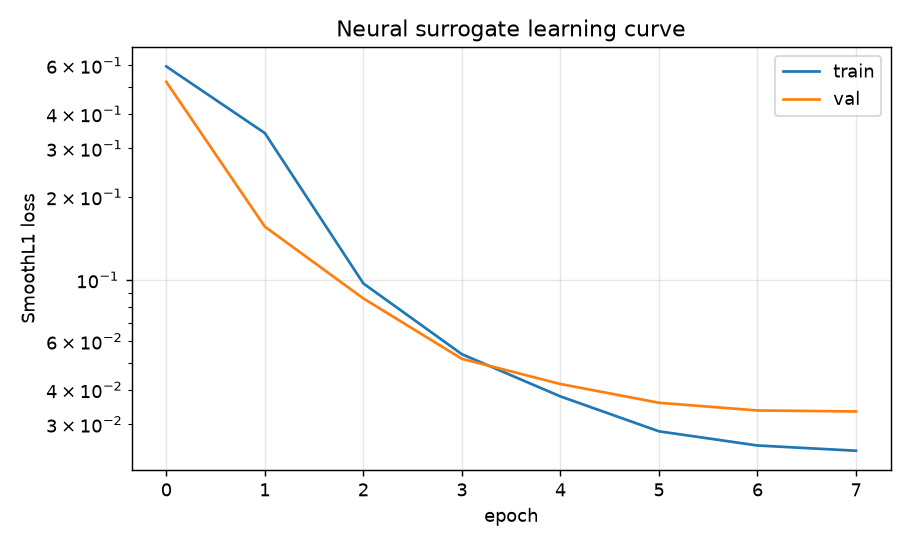
\includegraphics[width=0.9\linewidth]{figs/surrogate_learning_curve.png}
\caption{Surrogate learning curve (Smooth L1 Loss) showing training and validation convergence.}
\label{fig:surr_learning}
\end{figure}

\begin{figure}[htbp]
\centering
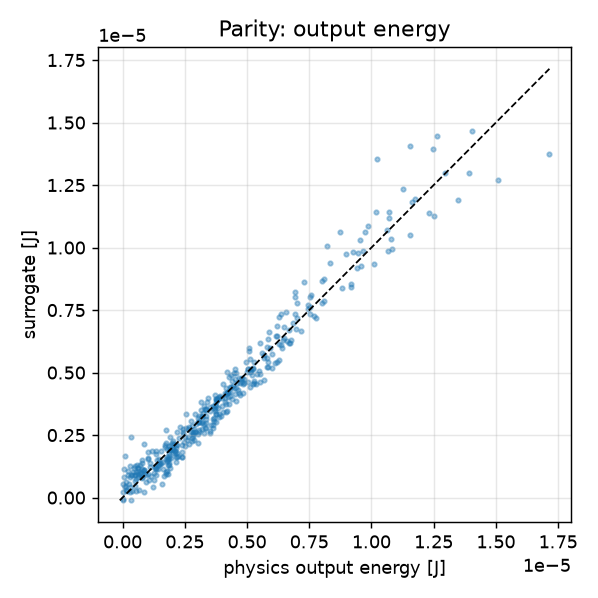
\includegraphics[width=0.9\linewidth]{figs/surrogate_parity_energy.png}
\caption{Parity plot of surrogate-predicted output energy vs. physics simulation.}
\label{fig:surr_parity}
\end{figure}

\subsection{SHG Conversion and AMP-4 Extrapolation}

The coupled-wave SHG model shows a peak conversion efficiency of \textbf{77.5\%} at an optimum crystal length of \textbf{11.7 mm}, yielding \textbf{992.3 mJ} of green 532 nm energy from the 1280 mJ of 1064 nm input, as shown in Fig.~\ref{fig:shg_curve}.

\begin{figure}[htbp]
\centering
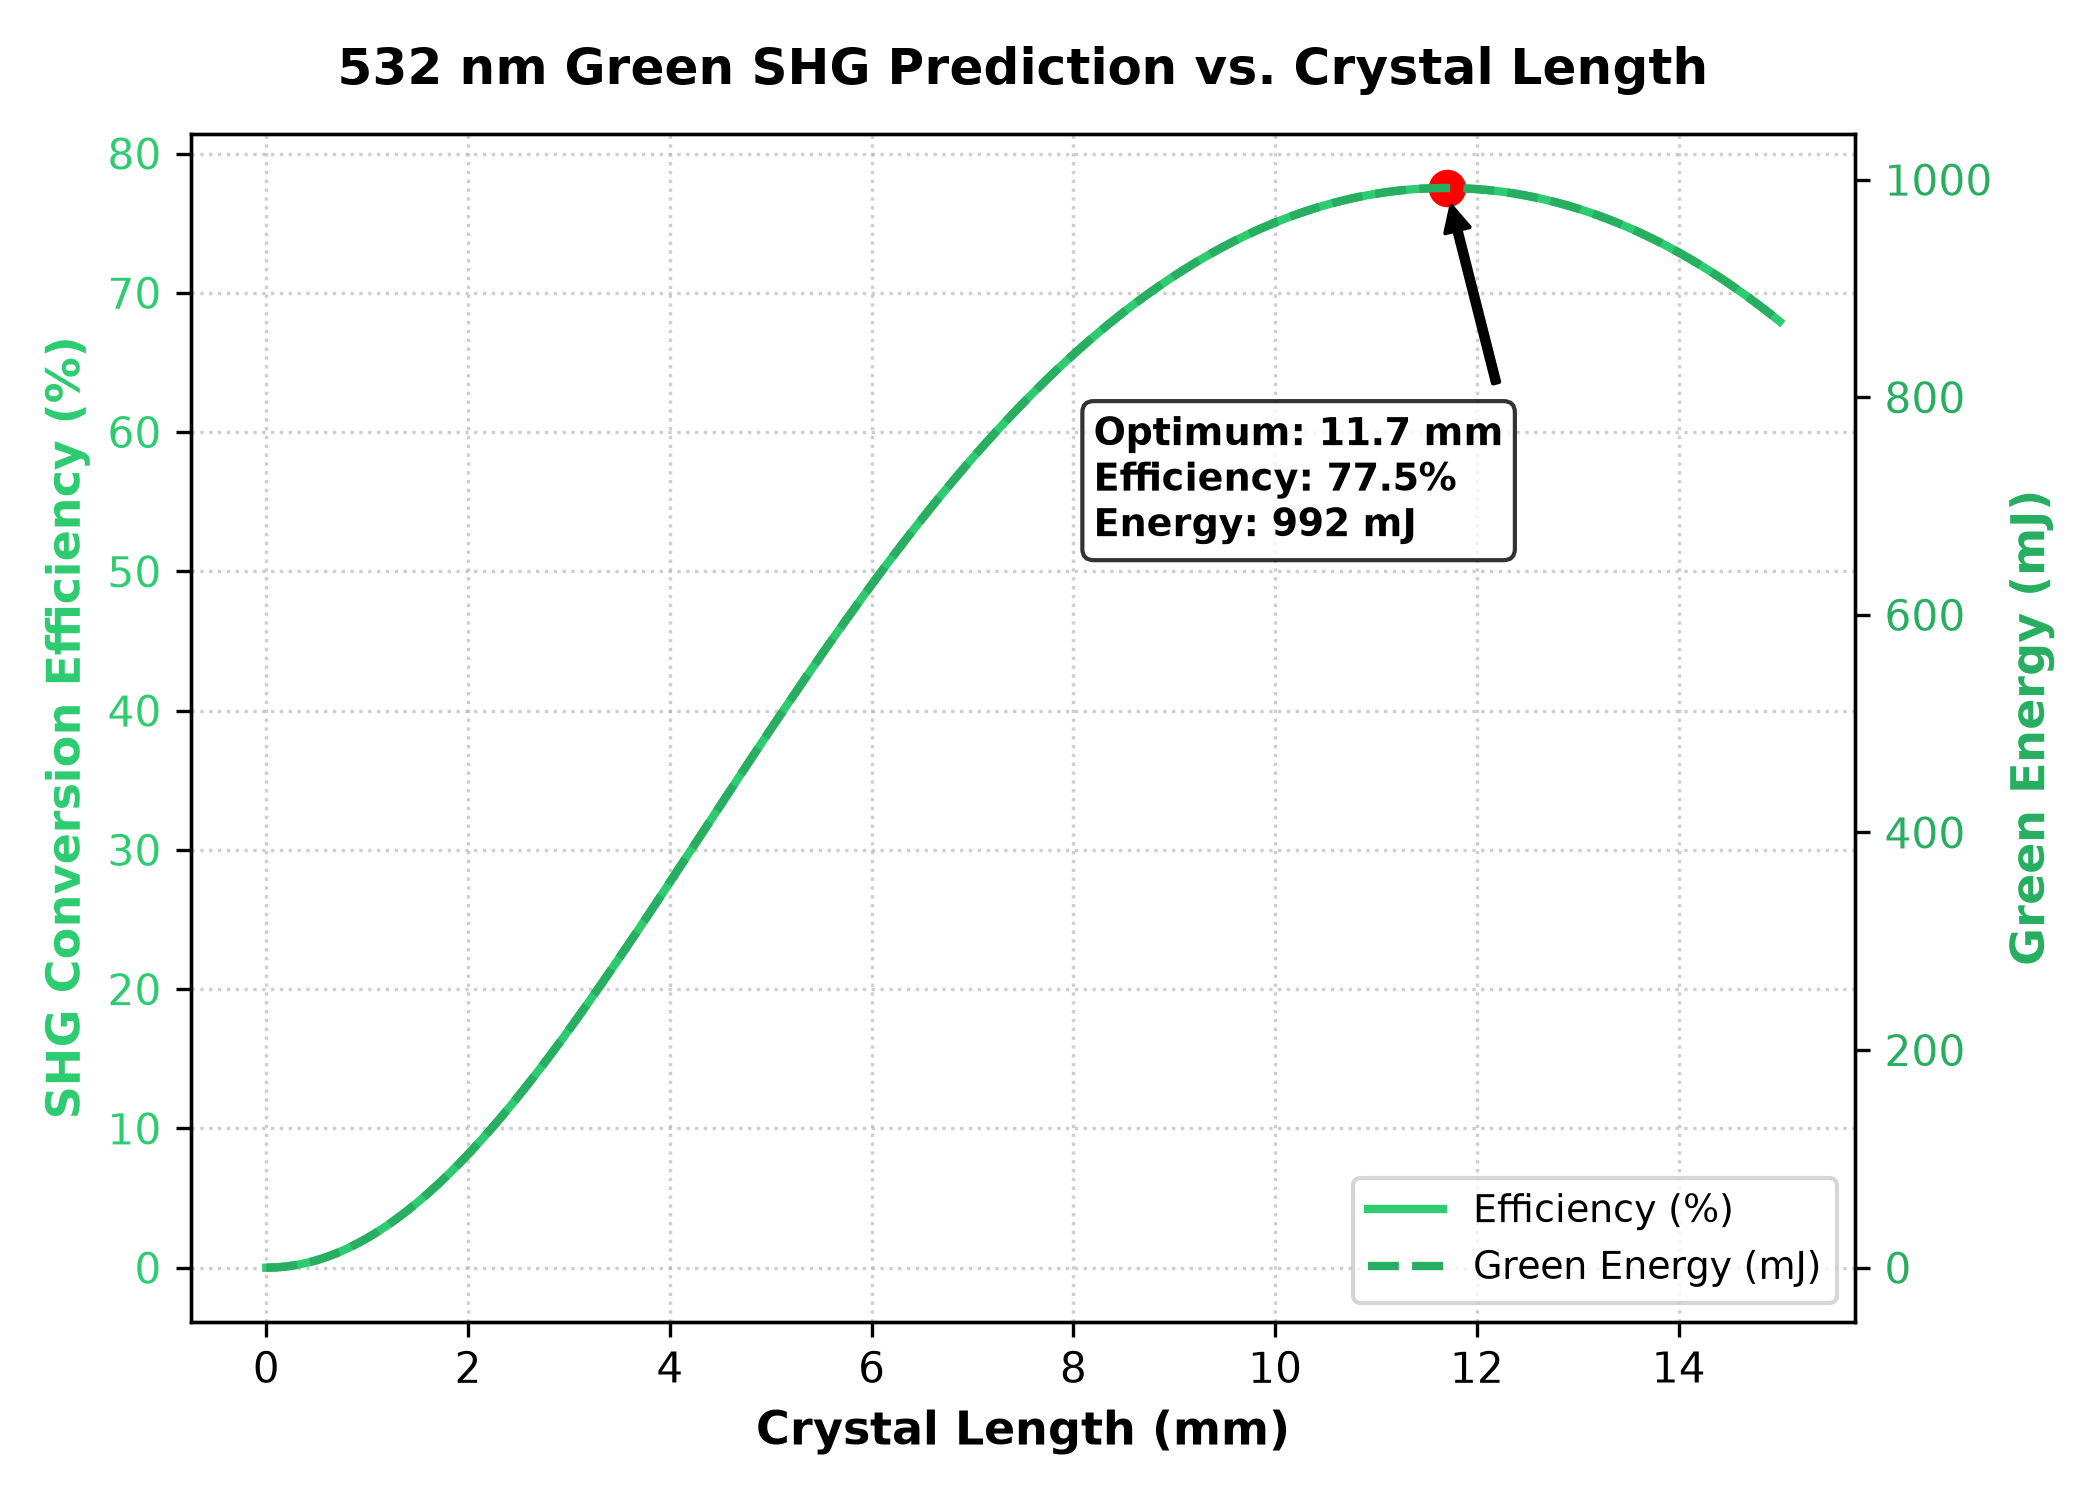
\includegraphics[width=0.9\linewidth]{figs/shg_curve.png}
\caption{SHG conversion efficiency curve vs. LBO crystal length.}
\label{fig:shg_curve}
\end{figure}

For a hypothetical fourth booster stage (AMP-4), the twin projects a peak output energy of \textbf{1571.9 mJ} (when seeded at 1.1672 J, gain 1.35) with a worst-case B-integral of 1.05 rad (B-safe). Optimizing the beam diameter schedule yields a B-integral reduction of \textbf{+49\%} (worst-stage B-integral reduced from 3.04 rad to 1.55 rad).

\begin{figure}[htbp]
\centering
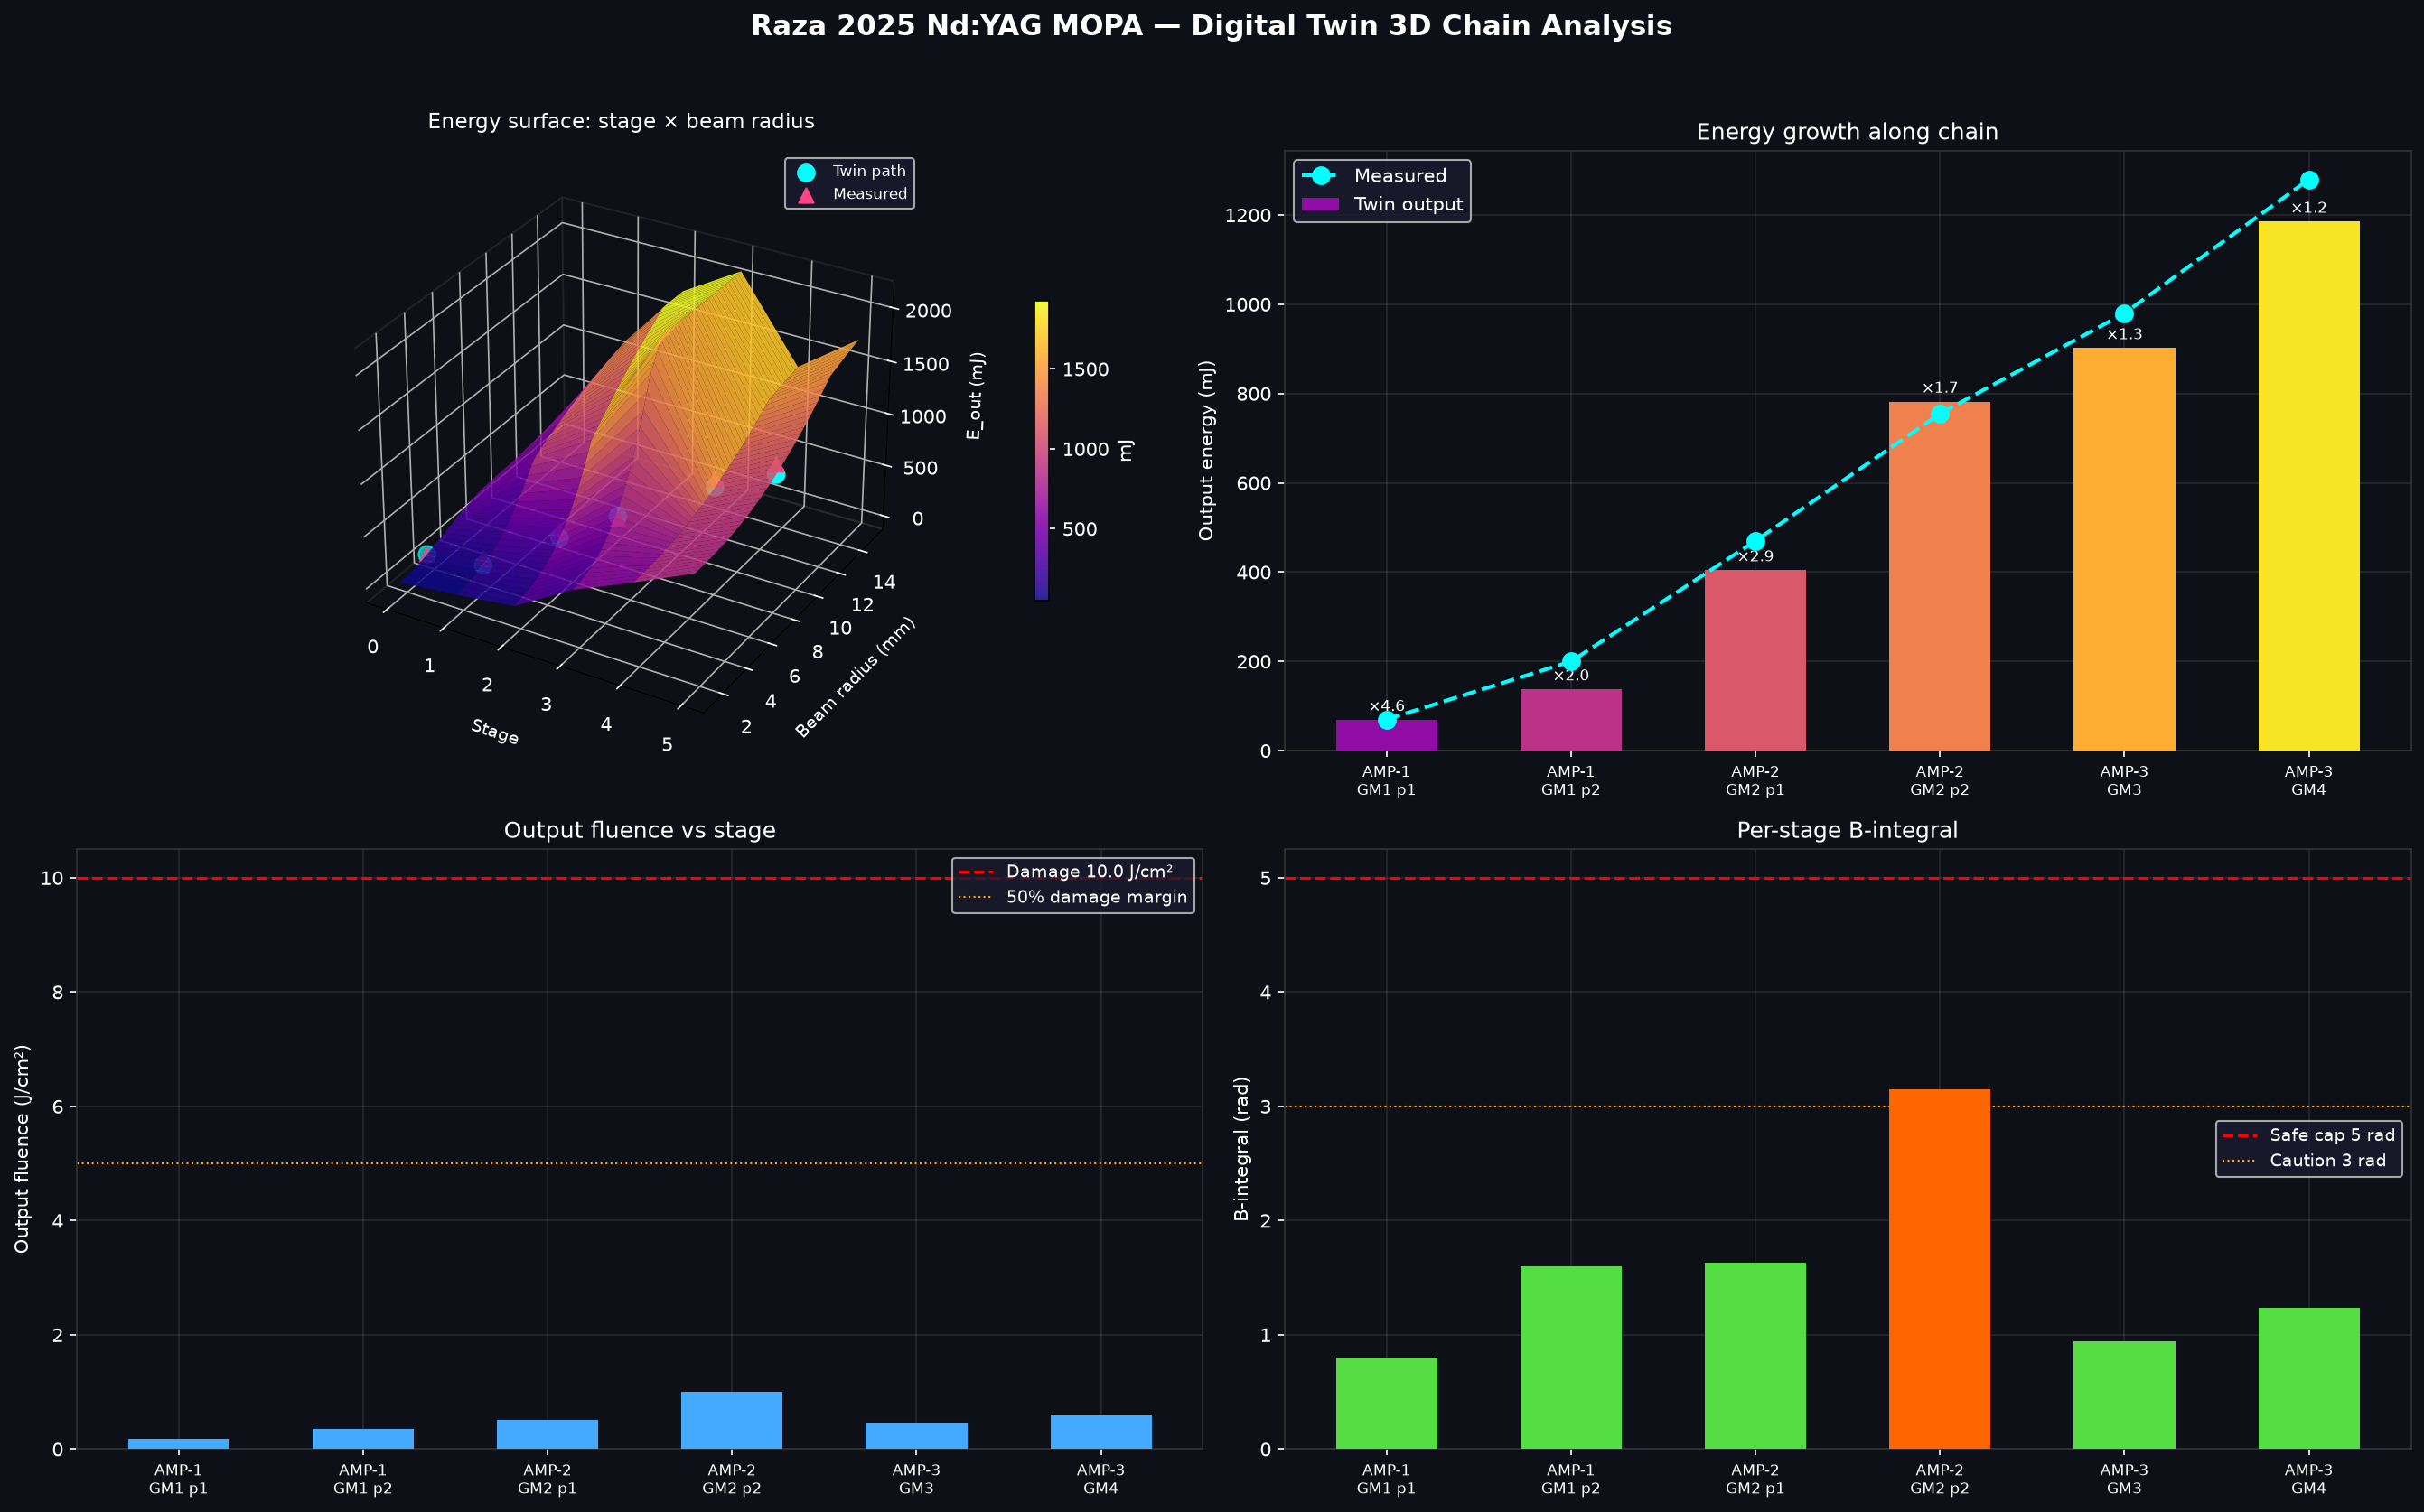
\includegraphics[width=0.9\linewidth]{figs/beam_3d.png}
\caption{3D beam propagation and B-integral growth along the amplifier chain.}
\label{fig:beam_3d}
\end{figure}

\subsection{Differentiable Inverse Design}

The target specifications and verification checks for the ensemble inverse design optimization are listed in Table~\ref{tab:inverse}. The recovered design parameters are: pump power $240.36\text{ W}$, crystal length $4.45\text{ cm}$, seed energy $3330.82\text{ nJ}$, residual GDD $24199.31\text{ fs}^2$, and SHG crystal length $12.56\text{ mm}$.

\begin{table}[htbp]
\centering
\caption{Inverse design target vs. physics check verification.}
\label{tab:inverse}
\begin{tabular}{lrrrr}
\toprule
Metric & Target & Surrogate & Physics & Diff \% \\
\midrule
Output Energy (J) & $6.00 \times 10^{-6}$ & $5.79 \times 10^{-6}$ & $5.76 \times 10^{-6}$ & 0.37\% \\
Pulse Duration (fs) & Free & 3330.73 & 3330.73 & 0.00\% \\
$M^2$ Beam Quality & 1.10 & 1.10 & 1.10 & 0.05\% \\
SHG Efficiency & 0.0100 & 0.0100 & 0.0099 & 0.79\% \\
Peak Power (W) & $1.50 \times 10^{6}$ & $1.62 \times 10^{6}$ & $1.63 \times 10^{6}$ & 0.27\% \\
\bottomrule
\end{tabular}
\end{table}

\section{Discussion \& Limitations}

While the saturation-dependent fill-factor model reduces the per-stage MAE to 10.88\% without any per-stage tuning, several limitations must be noted:
\begin{enumerate}
    \item \textbf{Single-System Tuning}: The transition parameter $\beta = 0.130$ was fitted specifically to the Raza et al. chain. While it generalizes reasonably to the Huang et al. system ($-18.8\%$ error), it yields large errors ($>50\%$) on other systems where internal stage details are absent.
    \item \textbf{Reporting Gaps in Literature}: The high errors in multi-system transfer (54.4\% MAE) are not due to model physics, but rather a reporting gap in the literature. Most publications omit critical per-stage details (e.g. beam-to-rod diameter ratio, stored energy, diode pump energy), making parameter-free MOPA validation difficult.
    \item \textbf{Parameter Sensitivity}: Leave-one-stage-out validation shows an MAE of 16.54\% (compared to 10.88\% full-fit), indicating a mild sensitivity to the training stage set.
\end{enumerate}

\section{Conclusion}

We have presented an open-source, physics-constrained digital twin of a joule-class multi-pass Nd:YAG MOPA chain. By incorporating a physically motivated saturation-dependent fill-factor correction, we match the accuracy of empirical calculations while avoiding per-stage tuning. The combination of this physical model with a high-fidelity deep neural surrogate enables rapid, constraint-aware inverse design with calibrated uncertainty bounds, providing a powerful instrument for the design and optimization of high-power laser chains.

\begin{acknowledgments}
The authors thank the High-Power Laser Lab team at NILORE for providing reference data and experimental insights. This work was supported in part by the National Institute of Lasers and Optronics.
\end{acknowledgments}

\bibliographystyle{apsrev4-2}
\bibliography{refs}

\end{document}
